\section{Θεωρητικό Υπόβαθρο}
\subsection{To μοντέλο Προγραμματισμού \en{OpenMP}}
\subparagraph{}
Το μοντέλο προγραμματισμού του \en{OpenMP} βασίζεται στο πολυνηματικό μοντέλο παραλληλισμού.  Η εφαρμογή ξεκινάει με ένα μόνο νήμα, το κύριο (\en{master thread}), που εκτελεί εντολές σειριακού κώδικα. Το \emph{\en{id}} αυτού του νήματος είναι πάντα μηδέν και η διάρκεια ζωής του είναι μέχρι το πέρας της εκτέλεσης του προγράμματος\cite{pdplab}. 

Όταν το κύριο νήμα  εισέρχεται στην περιοχή παράλληλου κώδικα (\en{parallel region}), τότε δημιουργούνται περισσότερα νήματα και το τμήμα αυτό εκτελείται ταυτόχρονα από τα παραγόμενα νήματα. Με την ολοκλήρωση της εκτέλεσης του παράλληλου τμήματος, όλα τα νήματα που δημιουργήθηκαν τερματίζουν και συνεχίζει μόνο το κύριο, μέχρι να βρεθεί κάποιο άλλο τμήμα παράλληλου κώδικα (\en{fork-join} μοντέλο)\cite{pdplab}. Το κύριο νήμα είναι υπεύθυνο για την δημιουργία των επιπλέον νημάτων για τη συνολική εκτέλεση. Τα νήματα που είναι ενεργά σε μια παράλληλη περιοχή αναφέρονται ως \en{"}ομάδα” (\emph{\en{thread team}}). Πάνω από μία ομάδες νημάτων μπορεί να είναι ενεργές ταυτόχρονα\cite{ompblaise}.

\begin{figure}[h]
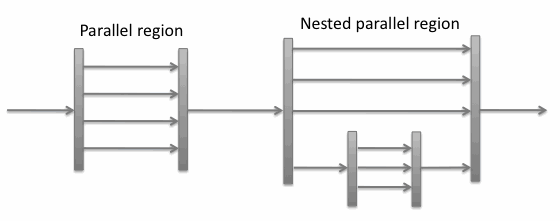
\includegraphics[width=\textwidth]{fork_join}
\captionsetup{justification=centering, singlelinecheck=false}
\caption{Κύριο νήμα και ομάδες νημάτων}
\label{fig:fork_join}
\end{figure}

\subsection{Αλληλεπίδραση νημάτων και περιβάλλοντος δεδομένων}
\subparagraph{}
Οπως προαναφέρθηκε, η εκτέλεση του προγράμματος ξεκινάει από το κύριο νήμα. Το νήμα αυτό συσχετίζεται με ένα περιβάλλον δεδομένων. Το περιβάλλον δεδομένων για ένα νήμα είναι ο χώρος διευθύνσεων μνήμης στον οποίο εισάγονται όλες οι μεταβλητές του προγράμματος, περιλαμβανομένων των \emph{καθολικών} μεταβλητών, των μεταβλητών που είναι αποθηκευμένες στη μνήμη \emph{\en{stack}} και αυτών που είναι αποθηκευμένες στη \emph{\en{heap}}\cite{book2}. 

Στο μοντέλο μνήμης του \en{OpenMP}, τα δεδομένα χωρίζονται σε δύο βασικές κατηγορίες μνήμης: στα ιδιωτικά(\emph{\en{private}}) και τα κοινόχρηστα(\emph{\en{shared}}).  Όλα τα νήματα έχουν πρόσβαση χωρίς περιορισμούς σε μεταβλητές που είναι αποθηκευμένες στην κοινόχρηστη μνήμη\cite{thenextstep7}.
\ \\
\begin{center}
\begin{figure}[h]
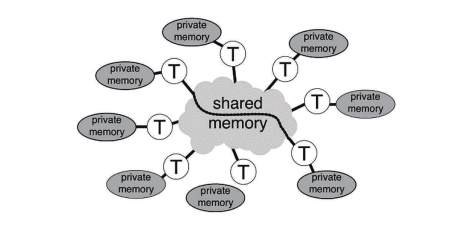
\includegraphics[width=\textwidth]{private_shared}
\captionsetup{justification=centering, singlelinecheck=false}
\caption{Μοντέλο μνήμης \en{OpenMP}}
\label{fig:private_shared}
\end{figure}
\end{center}
\ \\
\subsubsection{Ιδιωτική μνήμη}
\subparagraph{}
Πρόκειται για τη μνήμη που είναι προσβάσιμη και μπορεί να τροποποιηθεί από ένα μοναδικό νήμα. Τα νήματα δε μπορούν να έχουν πρόσβαση στην ιδιωτική μνήμη των υπόλοιπων νημάτων. Η διάρκεια ζωής μιας μεταβλητής στην ιδιωτική μνήμη είναι περιορισμένη και διαρκεί όσο εκτελείται ο παράλληλος κώδικας. Από προεπιλογή, κάθε ιδιωτική μεταβλητή δεν είναι αρχικοποιείται στην αρχή της παράλληλης περιοχής\cite{thenextstep9}.
\ \\
\ \\
\subsubsection{Κοινόχρηστη μνήμη}
\subparagraph{}
Εκτός από την ιδιωτική μνήμη, κάθε νήμα έχει πρόσβαση και σε ένα άλλο είδος μνήμης, την  κοινόχρηστη. Σε αντίθεση με την ιδιωτική, υπάρχει μόνο μία κοινόχρηστη μνήμη κατα τη διάρκεια εκτέλεσης του προγράμματος, και είναι προσπελάσιμη απο όλα τα νήματα. Ετσι, κάθε νήμα έχει την δυνατότητα τροποποίησης οποιασδήποτε μεταβλητής βρίσκεται στη κοινόχρηστη μνήμη.
Η ταυτόχρονη προσπέλαση κοινόχρηστης μνήμης από διαφορετικά νήματα, προκαλεί τα παρακάτω προβλήματα:
\clearpage
\paragraph{\en{Race Condition}}
\begin{center}
	\begin{minipage}[t]{0.45\linewidth}
\ \\
	Το φαινόμενο αυτό εμφανίζεται στις περιπτώσεις όπου μια ρουτίνα χρησιμοποιεί δεδομένα από τη κοινόχρηστη μνήμη. 
Αν η συνάρτηση καλείται παράλληλα, πολλά νήματα ενδέχεται να προσπαθήσουν να τροποποιήσουν ταυτόχρονα την ίδια διεύθυνση μνήμης, μέσω αυτής της ρουτίνας. Το φαινόμενο αυτό ονομάζεται \emph{\en{race condition}} και οδηγεί σε εσφαλμένους υπολογισμούς. Η απλούστερη λύση, ειναι η δημιουργία ιδιωτικού αντίγραφου για κάθε νήμα. Έτσι, πολλά νήματα μπορούν ταυτόχρονα να τροποποιούν δεδομένα που βρίσκονται σε διαφορετικές θέσεις μνήμης γιατί οι μεταβλητές ορίζονται στο ιδιωτικό περιβάλλον δεδομένων του κάθε νήματος.
	\end{minipage}
	\qquad
	\begin{minipage}[t]{0.47\linewidth}
		\selectlanguage{english}
		\begin{lstlisting}[tabsize=2, basicstyle=\small, language=C++, caption={\el{Παράδειγμα κώδικα με} race condition}, frame=tb]
#include <omp.h>

int main(void) {	
	int sum = 0;

	#pragma omp parallel for
	for (int i = 0;  i < 100; ++i) {
		sum += i;		
	}
}
\end{lstlisting}
\selectlanguage{english}
	\end{minipage}
\end{center}
\ \\
\paragraph{\en{False Sharing}}
\subparagraph{}
Το \emph{\en{false sharing}} είναι ένα συχνό πρόβλημα στην παράλληλη επεξεργασία κοινόχρηστης μνήμης. Εμφανίζεται όταν δύο ή περισσότεροι πυρήνες κρατούν αντίγραφο της ίδιας γραμμής προσωρινής μνήμης (\emph{\en{cache}}). 

\begin{figure}[h]
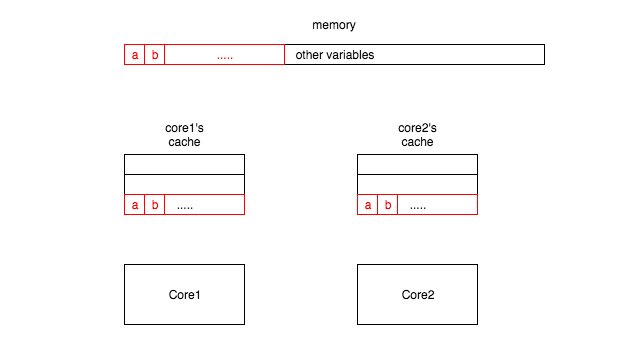
\includegraphics[width=0.5\textwidth]{false_sharing_2}
\centering
\captionsetup{justification=centering, singlelinecheck=false}
	\caption{\en{False sharing (1/3)}}
\label{fig:false_sharing_2}
\end{figure}

\ \\
\begin{wrapfigure}{l}{0.5\textwidth}
	\centering
	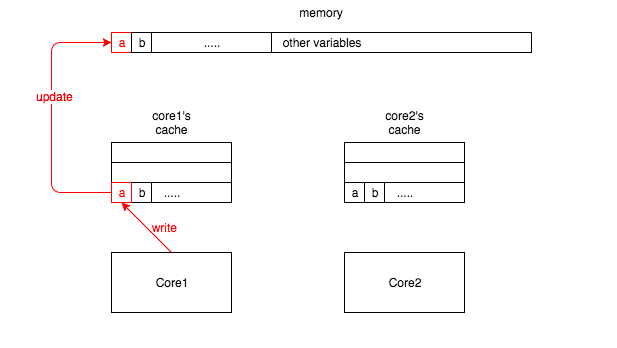
\includegraphics[width=0.5\textwidth]{false_sharing_3}
	\captionsetup{justification=centering, singlelinecheck=false}
	\caption{\en{False sharing (2/3)}}
\label{fig:false_sharing_3}
\end{wrapfigure}

Οταν ένα νήμα τροποποιεί μια μεταβλητή, η γραμμή της μνήμης που βρίσκεται η μεταβλητή ακυρώνεται στους υπόλοιπους πυρήνες. Η γραμμή μνήμης θα πρέπει να ακυρωθεί ακόμη και αν ένας πυρήνας μπορεί να μη τροποποιεί τη συγκεκριμένη θέση μνήμης, αλλά να θέλει να τροποποιήσει ένα άλλο δεδομένο που βρίσκεται σε αυτ. 
\ \\
\ \\
\ \\
\begin{wrapfigure}{l}{0.55\textwidth}
	\centering
	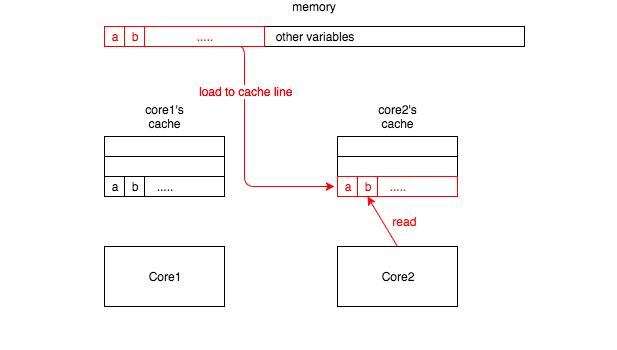
\includegraphics[width=0.55\textwidth]{false_sharing_4}
	\captionsetup{justification=centering, singlelinecheck=false}
	\caption{\en{False sharing (3/3)}}
\label{fig:false_sharing_4}
\end{wrapfigure}

Ο δεύτερος πυρήνας θα πρέπει να φορτώσει εκ νέου τη γραμμή μνήμης, προτού αποκτήσει ξανά πρόσβαση στα δεδομένα της. Η προσπέλαση δεδομένων της κοινόχρηστης μνήμης συχνά επηρεάζει την απόδοση του προγράμματος\cite{false_sharing}.
Λύση στο πρόβλημα του \en{false sharing}, αποτελεί η εισαγωγή τεχνητού κενού (\en{padding}) ανάμεσα στα δεδομένα της γραμμής, με σκοπό την τοποθέτησή τους σε ξεχωριστές γραμμές μνήμης.
\clearpage
\subsection{Μοντέλο συνοχής μνήμης}
\subparagraph{}
Για την αποφυγή φαινομένων \en{race condition} που οδηγούν σε λανθασμένα αποτελέσματα, απαιτείται συχνά ο συντονισμός πρόσβασης των νημάτων στις μεταβλητές της κοινόχρηστης μνήμης. Ο όρος \emph{"συγχρονισμός"} αναφέρεται στους μηχανισμούς συντονισμού των νημάτων. Οι μέθοδοι συγχρονισμού εγγυώνται το διάβασμα της σωστής τιμής μια μεταβλητής στην κοινόχρηστη μνήμη μετά από οποιαδήποτε ενημέρωσή της. Μηχανισμοί συγχρονισμού ειναι οι\cite{book2_23} εξής:
\selectlanguage{english}
\begin{itemize}
    \item {\#}pragma omp critical 
    \item {\#}pragma omp atomic
    \item {\#}pragma omp barrier 
    \item {\#}pragma omp ordered
    \item {\#}pragma omp flush
\end{itemize}
\selectlanguage{greek}

\subsection{Οδηγίες διαμοιρασμού εργασίας}
\subparagraph{}
Η εντολή \en{{\#}pragma omp parallel} κατασκευάζει ένα \en{SPMD} πρόγραμμα (\en{"Single Program Multiple Data"}) οπου κάθε νήμα εκτελεί τον ίδιο κώδικα. Ο όρος \emph{"oδηγία διαμοιρασμού εργασίας"} (\en{worksharing construct}) χρησιμοποιείται για να περιγραφεί η κατανομή της εκτέλεσης της αντίστοιχης περιοχής μεταξύ των νημάτων μιας ομάδας που τη συναντά.

Μια οδηγιά διαμοιρασμού εργασίας δεν έχει κανένα εμπόδιο συγχρονισμού(“\en{barrier}”) κατά την είσοδο. Ωστόσο υπάρχει ένα σιωπηρό εμπόδιο στο τέλος της οδηγίας. Το εμπόδιο μπορεί να αναιρεθεί με τη χρήση της \emph{"φράσης"} \en{(clause)} \emph{nowait}. Εάν υπάρχει, το πρόγραμμα μπορεί να παραλείψει το εμπόδιο στο τέλος της οδηγίας. Σε αυτή την περίπτωση, τα νήματα που τελειώνουν νωρίτερα μπορούν να προχωρήσουν στις υπόλοιπες οδηγίες που ακολουθούν στην παράλληλη περιοχή\cite{openmpse16}.

\ \\
\ \\
\subsubsection{Οδηγία διαμοιρασμού εργασίας βρόγχου - \en{for}}
\subparagraph{}
Η οδηγία διαμοιρασμού εργασίας βρόγχου καθορίζει ότι οι επαναλήψεις ενός ή περισσότερων βρόχων θα εκτελούνται παράλληλα από μια ομάδα νημάτων. Οι επαναλήψεις διανέμονται στα ήδη υπάρχοντα νήματα της ομάδας νημάτων της παράλληλης περιοχής.
\ \\
\selectlanguage{english}
\begin{lstlisting}[language=C++, caption={\el{Σύνταξη οδηγίας διαμοιρασμού εργασίας βρόγχου}} , frame=tlrb]{Name}
#pragma omp for [clause[[,]clause]...] new-line
	for-loops
\end{lstlisting}
\clearpage
\begin{lstlisting}[language=C++, caption={\el{Αποδεκτές φράσεις οδηγίας} for} , frame=tlrb]{Name}
private(list)
firstprivate(list)
lastprivate([lastprivate-modifier:]list)
linear(list[:linear-step])
reduction([reduction-modifier,]reduction-identifier : list)
schedule([modifier[, modifier]:]kind[, chunk_size])
collapse(n)
ordered[(n)]
allocate([allocator :]list)
order(concurrent)
\end{lstlisting}
\selectlanguage{greek}


\subsubsection{Οδηγία \en{sections}}
\subparagraph{}

      Η οδηγία \en{sections} είναι μια μη επαναληπτική περιοχή διαμοιρασμού εργασίας. Καθορίζει ότι τα εσωκλειώμενα τμήματα κώδικα θα διαμοιραστούν μεταξύ των νημάτων της ομάδας. Μια οδηγία \en{sections} μπορεί να περιέχει περισσότερες από μία, ανεξάρτητες, οδηγίες section. Κάθε τμήμα εκτελείται μια φορά από ένα νήμα της ομάδας, ενώ διαφορετικά τμήματα εκτελούνται από διαφορετικά νήματα. Η σύνταξη μιας οδηγίας sections φαίνεται παρακάτω\cite{pdplab}

\selectlanguage{english}
\begin{lstlisting}[language=C++, caption={\el{Σύνταξη οδηγίας} sections} , frame=tlrb]{Name}
#pragma omp sections [clause[ [,] clause] ... ] new-line 
   { 
   [#pragma omp section new-line] 
      structured-block 
   [#pragma omp section new-line 
      structured-block] 
   ... 
   }
\end{lstlisting}

\begin{lstlisting}[language=C++, caption={\el{Αποδεκτές φράσεις οδηγίας} sections} , frame=tlrb]{Name}
private(list) 
firstprivate(list) 
lastprivate([ lastprivate-modifier:] list) 
reduction([reduction-modifier ,] reduction-identifier : list) 
allocate([allocator :] list) 
nowait
\end{lstlisting}
\selectlanguage{greek}

\subsubsection{Οδηγία \en{single}}
\subparagraph{}
Η οδηγία \en{single} καθορίζει ότι το μπλοκ εκτελείται από ένα μόνο νήμα της ομάδας (όχι απαραίτητα το κύριο νήμα). Τα άλλα νήματα της ομάδας, τα οποία δεν εκτελούν το μπλοκ που βρίσκεται μέσα στην οδηγία single, περιμένουν σε ένα υπονοούμενο φράγμα στο τέλος της οδηγίας \en{single}, εκτός εάν έχει οριστεί η φράση \en{nowait} \cite{openmpse16}.

\selectlanguage{english}
\begin{lstlisting}[language=C++, caption={\el{Σύνταξη οδηγίας} single} , frame=tlrb]{Name} 
#pragma omp single [clause[ [,] clause] ... ] new-line 
   structured-block
\end{lstlisting}

\begin{lstlisting}[language=C++, caption={\el{Αποδεκτές φράσεις οδηγίας} sections} , frame=tlrb]{Name}
private(list) 
firstprivate(list) 
copyprivate(list) 
allocate([allocator :] list) 
nowait
\end{lstlisting}
\selectlanguage{greek}

\clearpage
\subsection{Φράσεις - \en{Clauses}}
\subparagraph{}
Δεδομένου οτι το \en{OpenMP} είναι ένα μοντέλο προγραμματισμού κοινής μνήμης, οι περισσότερες μεταβλητές στον κώδικα \en{OpenMP} είναι ορατές σε όλα τα νήματα από προεπιλογή. Οι ιδιωτικές μεταβλητές χρησιμοποιούνται για να αποφευχθούν τα \en{race conditions} και υπάρχει ανάγκη μεταβίβασης τιμών μεταξύ σειριακού κώδικα και παράλληλης περιοχής. Η διαχείριση αυτή των δεδομένων επιτυγχάνεται με τις φράσεις \emph{\en{(clauses)}}. Οι βασικότερες ομάδες διαχωρισμού φράσεων αναφέρονται στα επόμενα κεφάλαια.

\subsubsection{Φράσεις διαμοιρασμού δεδομένων - \en{Data sharing attribute clauses}}
\subparagraph{}
Οι φράσεις διαμοιρασμού δεδομένων χρησιμοποιούνται σε οδηγίες για να δίνουν στο χρήστη τη δυνατότητα έλεγχου των δεδομένων που χρησιμοποιούνται στην οδηγία.

\paragraph{Φράση \en{shared}}
\subparagraph{}
Τα δεδομένα που δηλώνονται εκτός μιας παράλληλης περιοχής, ειναι διαμοιραζόμενες σε όλα τα νήματα. Αν η μεταβλητή τροποποιηθεί από ένα νήμα, η αλλαγή θα είναι ορατή από όλα τα νήματα. Οι μεταβλητές με αυτό το χαρακτηριστικό διατηρούν την τιμή τους και μετά την έξοδο από το παράλληλο μπλοκ.

\paragraph{Φράση \en{private}}
\subparagraph{}
Τα δεδομένα που δηλώνονται σε μια παράλληλη περιοχή είναι ιδιωτικά για κάθε νήμα. Ετσι, κάθε νήμα θα έχει ένα τοπικό αντίγραφο και θα το χρησιμοποιεί ως προσωρινή μεταβλητή. Μια ιδιωτική μεταβλητή δεν έχει αρχικοποιηθεί και η τιμή δεν διατηρείται για χρήση εκτός της παράλληλης περιοχής.

\paragraph{Φράση \en{default}}
\subparagraph{}
Επιτρέπει στο χρήστη να δηλώσει ότι η προεπιλογή για τα δεδομένα σε μια παράλληλη περιοχή θα είναι ή κοινόχρηστα ή \emph{\en{none}} για \en{C} / \en{C}++ ή {\en{firstprivate}}. Η επιλογή none αναγκάζει τον χρήστη να δηλώνει κάθε μεταβλητή στην παράλληλη περιοχή χρησιμοποιώντας φράσης διαμοιρασμού μνήμης.

\paragraph{Φράση \en{firstprivate}}
\subparagraph{}
Η μόναδική διαφορά της από τη φράση \en{private} είναι οτι σε αντίθεση με τη \en{private}, η μεταβλητή αρχικοποιείται χρησιμοποιώντας την τιμή της μεταβλητής με το ίδιο όνομα που έχει και η μεταβλητή του κύριου νήματος.

\paragraph{Φράση \en{lastprivate}}
\subparagraph{}   

Η μοναδική διαφορά της από τη φράση \en{private} είναι ότι σε αντιθεση με τη private, η αρχική τιμή ανανεώνεται μετά το construct. Μια μεταβλητή μπορεί να είναι και firstprivate και lastprivate.


\paragraph{Φράση \en{threadprivate}}
\subparagraph{}
      Η φράση \en{threadprivate} καθορίζει ότι καθολικά αντικείμενα (ή μεταβλητές) μπορούν να γίνουν προσωρινά ιδιωτικά για κάποιο νήμα. Με αυτό τον τρόπο, μπορούμε να ορίσουμε καθολικά αντικείμενα, αλλά να μετατρέψουμε την εμβέλειά τους και να τα κάνουμε τοπικά για κάποιο νήμα. Οι μεταβλητές για τις οποίες ισχύει η φράση \en{threadprivate} συνεχίζουν να είναι ιδιωτικές, για κάθε νήμα, ακόμα και σε διαφορετικές παράλληλες περιοχές\cite{pdplab}.

\paragraph{Φράση \en{reduction}}
\subparagraph{}    
\selectlanguage{english}
\begin{lstlisting}[language=C++, caption={\el{Σύνταξη οδηγίας διαμοιρασμού εργασίας βρόγχου}} , frame=tlrb]{Name}
 reduction(operator | intrinsic : list):\end{lstlisting}
\selectlanguage{greek} 
    

Η φράση αυτή εκτελεί μία πράξη αναγωγής σε κάποιες μοιραζόμενες μεταβλητές . Όλες οι μεταβλητές που βρίσκονται σε μία παράλληλη περιοχή και υπάρχουν στη λίστα της φράσης reduction, αντιγράφονται σε τοπικά αντίγραφα, ένα για κάθε νήμα. Με την ολοκλήρωση των επαναλήψεων, εφαρμόζεται η πράξη που ορίζεται στο πεδίο \emph{\en{operator}} και το τελικό αποτέλεσμα αποθηκεύεται στην αρχική θέση τους\cite{pdplab}.

\subsubsection{Φράσεις συγχρονισμού - \en{Data sharing attribute clauses}}
\subparagraph{}
Χρησιμοποιούνται για να αποφευχθούν προβλήματα \emph{\en{race condition}} σε κοινόχρηστα δεδομένα.

\paragraph{Φράση \en{critical}} 
\subparagraph{}
Το μπλοκ κώδικα που περικλείεται, εκτελείται μόνο από ένα νήμα κάθε φορά και όχι ταυτόχρονα από πολλά νήματα. Χρησιμοποιείται συχνά για την προστασία κοινόχρηστων δεδομένων από \emph{\en{race conditions}}.

\paragraph{Φράση \en{atomic}}
\subparagraph{}
H ενημέρωση μνήμης (εγγραφή ή ανάγνωση-τροποποίηση-εγγραφή) στην επόμενη οδηγία θα εκτελεστεί ατομικά. Δεν καθιστά ολόκληρη στην έκφραση \emph{\en{atomic}} αλλα μόνο την ενημέρωση μνήμης. Ένας μεταγλωττιστής μπορεί να χρησιμοποιεί ειδικές οδηγίες \en{hardware} για καλύτερη επίδοση από ό,τι όταν χρησιμοποιεί το \en{critical clause}.
      
      
\paragraph{Φράση \en{ordered}}
\subparagraph{}
To μπλοκ εκτελείται με τη σειρά με την οποία οι επαναλήψεις θα εκτελούνταν σε σειριακό βρόχο.

\paragraph{Φράση \en{barrier}}
\subparagraph{}
Kάθε νήμα περιμένει έως ότου όλα τα άλλα νήματα μιας ομάδας φτάσουν σε αυτό το σημείο. Η οδηγία διαμοιρασμού εργασιών έχει έναν σιωπηρό συγχρονισμό με \emph{\en{barrier}} στο τέλος της.
\clearpage
\paragraph{Φράση \en{nowait}}
\subparagraph{}
Καθορίζει ότι τα νήματα που ολοκληρώνουν την εργασία τους μπορούν να προχωρήσουν χωρίς να περιμένουν να τελειώσουν όλα τα νήματα της ομάδας. Ελλείψει αυτής της φράσης, τα νήματα συγχρονίζονται με \emph{\en{barrier}} στο τέλος της οδηγίας διαμοιρασμού εργασιών.

\subsubsection{Φράσεις \en{scheduling}}
\subparagraph{}
      Χρησιμοποιείται στην οδηγία διαμοιρασμού εργασίας βρόγχου. Οι επαναλήψεις της οδηγίας ανατίθενται σε κάθε νήμα σε ένα σύμφωνα με τον \emph{τύπο} που ορίζεται στην φράση αυτή.
\selectlanguage{english}
\begin{lstlisting}[language=C++, caption={\el{Σύνταξη οδηγίας διαμοιρασμού εργασίας βρόγχου}} , frame=tlrb]{Name}
schedule(type, chunk): 
\end{lstlisting}
\selectlanguage{greek}
\ \\
    •  Οι τρεις τύποι προγραμματισμού είναι:\\
      
    \textbf{1. \en{static}}:
    \subparagraph{}

       Οι επαναλήψεις κατανέμονται σε κάθε νήμα πριν την εκτέλεση της λουπας, και χωρίζονται ισόποσα σε όλα τα threads. Παρόλα αυτά ο καθορισμός ενός ακεραίου αναθέτει ένα συγκεκριμένο αριθμό επαναλήψεων για ένα συγκεκριμένο νήμα.\\
       
    \textbf{2. \en{dynamic}}: 
    \subparagraph{}
       Ορισμένες από τις επαναλήψεις κατανέμονται σε μικρό αριθμό νημάτων. Μόλις ένα συγκεκριμένο νήμα ολοκληρώσει την εκχωρημένη επανάληψή του, επιστρέφει για να πάρει μία από τις επαναλήψεις που απομένουν. Το ακέραιο όρισμα καθορίζει τον αριθμό των συνεχόμενων επαναλήψεων που εκχωρούνται σε ένα νήμα κάθε φορά.\\
\clearpage
    \textbf{3. \en{guided}}: 
    \subparagraph{}
       Ενας μεγάλος αριθμός από συνεχείς επαναλήψεις ανατίθεται σε κάθε νήμα δυναμικά. Το μέγεθος των επαναλήψεων μειώνεται εκθετικά με κάθε διαδοχική κατανομή σε ένα ελάχιστο μέγεθος που καθορίζεται στο κομμάτι της παραμέτρου.\\
       
       
       \begin{figure}[h]
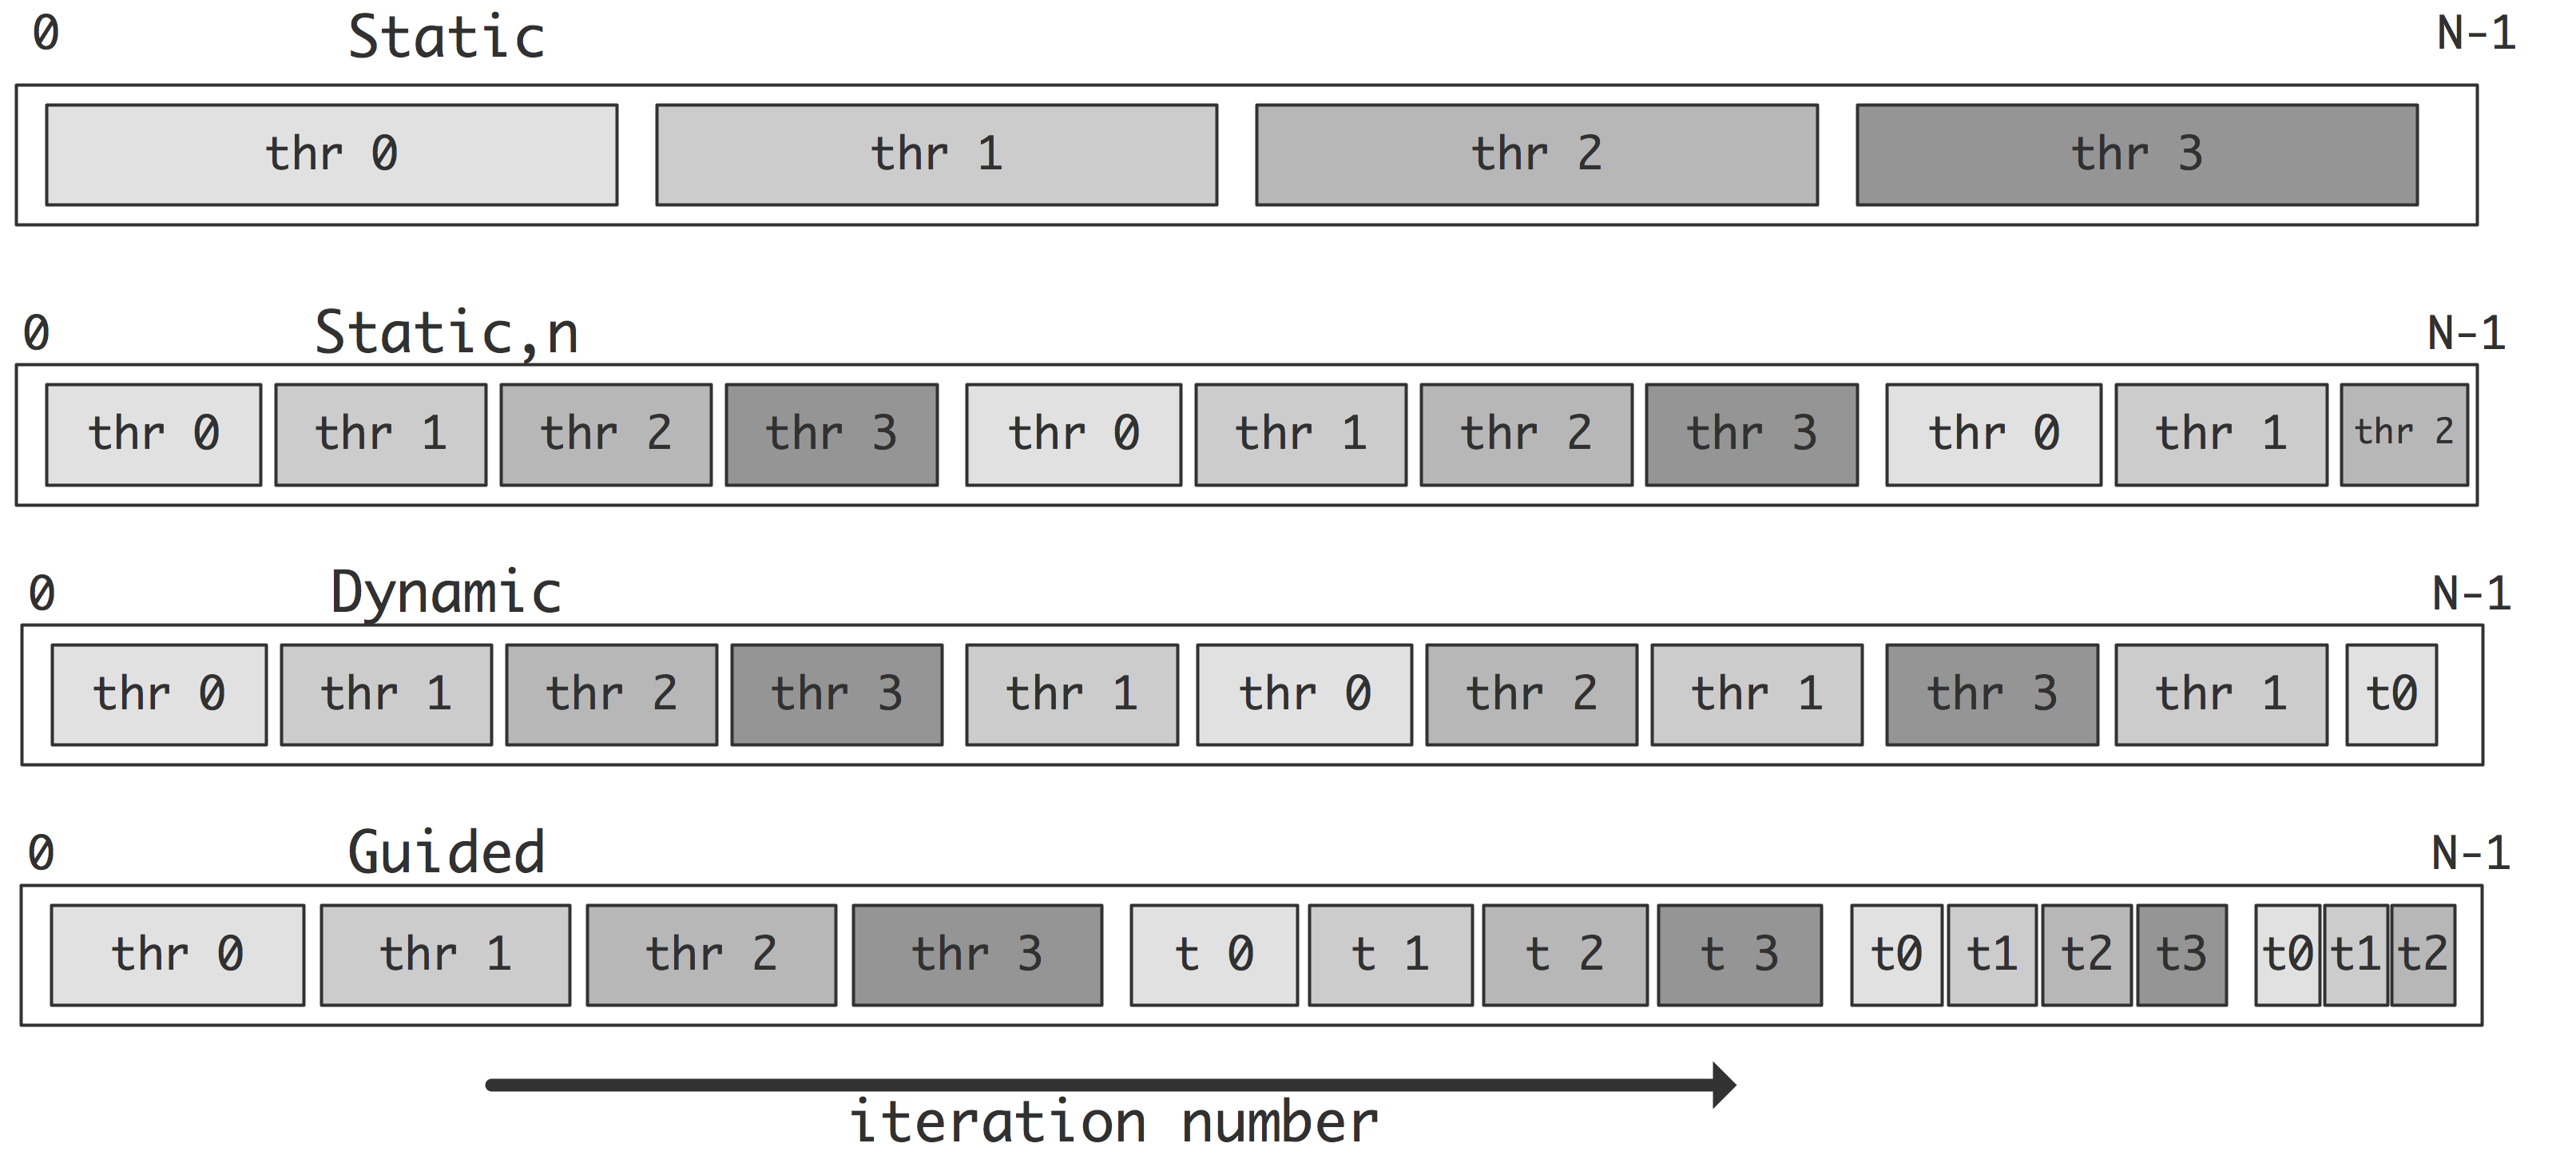
\includegraphics[width=\textwidth]{schedules}
\centering
\captionsetup{justification=centering, singlelinecheck=false}
	\caption{Τύποι φράσης \en{Schedule}}
\label{fig:schedules}
\end{figure}


\subsubsection{Αλλες φράσεις}
\subparagraph{}
\subsubsection{Φράσεις \en{flush}}
\subparagraph{}
Η τιμή αυτής της μεταβλητής αποθηκεύεται απο την register στη μνήμη, για χρήση της εκτός της παράλληλης περιοχής.
\subsubsection{Φράσεις \en{master}}
\subparagraph{}
      Εκτελείται μόνο από το κύριο νήμα. Δεν υπάρχει υπονοούμενο barrier. Τα υπόλοιπα νήματα θα συνεχίσουν τους υπολογισμούς.

{\Large TODO mporo na valo ena kefalaio gia ENVIRONMENTAL VALUES \\
TODO  Μπορώ να βάλω ενα κεφάλειο για τα runtime functions.}
